\documentclass[compress]{beamer}
\mode<presentation>
\usetheme{Warsaw}
\usecolortheme{seagull}
%\useoutertheme[subsection=false]{smoothbars}
\useoutertheme{infolines}
\useinnertheme{rectangles}

\setbeamercovered{dynamic}

\usepackage{array}
\usepackage{amsmath,amssymb,amsfonts,mathrsfs,amsthm}
\usepackage[utf8]{inputenc}
\usepackage{listings}
\usepackage{mathtools}
\usepackage{dsfont}
\usepackage{pdfpages}
\usepackage[textsize=footnotesize,color=green]{todonotes}
\usepackage{algorithm, algorithmic}
\usepackage{bm}
\usepackage{tikz}
\usepackage[normalem]{ulem}

\usepackage{graphicx}
\usepackage{subfigure}
%\usepackage{caption}
%\usepackage{subcaption}

\usepackage{color}
\usepackage{undertilde}
\usepackage{pdflscape}
\usepackage{pifont}

\usepackage{bibentry}
\nobibliography*

%\usepackage[osf]{mathpazo}
%\usepackage{mathpazo}
%\renewcommand\rmdefault{ptm}

\renewcommand{\topfraction}{0.85}
\renewcommand{\textfraction}{0.1}
\renewcommand{\floatpagefraction}{0.75}

\newcommand{\vect}[1]{\ensuremath\boldsymbol{#1}}
\newcommand{\tensor}[1]{\underline{\vect{#1}}}
\newcommand{\del}{\triangle}
\newcommand{\grad}{\nabla}
\newcommand{\curl}{\grad \times}
\renewcommand{\div}{\grad \cdot}
\newcommand{\ip}[1]{\left\langle #1 \right\rangle}
\newcommand{\eip}[1]{a\left( #1 \right)}
\newcommand{\pd}[2]{\frac{\partial#1}{\partial#2}}
\newcommand{\pdd}[2]{\frac{\partial^2#1}{\partial#2^2}}

\newcommand{\circone}{\ding{192}}
\newcommand{\circtwo}{\ding{193}}
\newcommand{\circthree}{\ding{194}}
\newcommand{\circfour}{\ding{195}}
\newcommand{\circfive}{\ding{196}}

\newcommand{\Reyn}{\rm Re}

\newcommand{\bs}[1]{\boldsymbol{#1}}
\DeclareMathOperator{\diag}{diag}

\newcommand{\equaldef}{\stackrel{\mathrm{def}}{=}}

\newcommand{\tablab}[1]{\label{tab:#1}}
\newcommand{\tabref}[1]{Table~\ref{tab:#1}}

\newcommand{\theolab}[1]{\label{theo:#1}}
\newcommand{\theoref}[1]{\ref{theo:#1}}
\newcommand{\eqnlab}[1]{\label{eq:#1}}
\newcommand{\eqnref}[1]{\eqref{eq:#1}}
\newcommand{\seclab}[1]{\label{sec:#1}}
\newcommand{\secref}[1]{\ref{sec:#1}}
\newcommand{\lemlab}[1]{\label{lem:#1}}
\newcommand{\lemref}[1]{\ref{lem:#1}}

\newcommand{\mb}[1]{\mathbf{#1}}
\newcommand{\mbb}[1]{\mathbb{#1}}
\newcommand{\mc}[1]{\mathcal{#1}}
\newcommand{\nor}[1]{\left\| #1 \right\|}
\newcommand{\snor}[1]{\left| #1 \right|}
\newcommand{\LRp}[1]{\left( #1 \right)}
\newcommand{\LRs}[1]{\left[ #1 \right]}
\newcommand{\LRa}[1]{\left\langle #1 \right\rangle}
\newcommand{\LRc}[1]{\left\{ #1 \right\}}
\newcommand{\tanbui}[2]{\textcolor{blue}{\sout{#1}} \textcolor{red}{#2}}
\newcommand{\Grad} {\ensuremath{\nabla}}
\newcommand{\Div} {\ensuremath{\nabla\cdot}}
\newcommand{\Nel} {\ensuremath{{N^\text{el}}}}
\newcommand{\jump}[1] {\ensuremath{\LRs{\![#1]\!}}}
\newcommand{\uh}{\widehat{u}}
\newcommand{\fnh}{\widehat{f}_n}
\renewcommand{\L}{L^2\LRp{\Omega}}
\newcommand{\pO}{\partial\Omega}
\newcommand{\Gh}{\Gamma_h}
\newcommand{\Gm}{\Gamma_{-}}
\newcommand{\Gp}{\Gamma_{+}}
\newcommand{\Go}{\Gamma_0}
\newcommand{\Oh}{\Omega_h}

\newcommand{\eval}[2][\right]{\relax
  \ifx#1\right\relax \left.\fi#2#1\rvert}

\def\etal{{\it et al.~}}


\def\arr#1#2#3#4{\left[
\begin{array}{cc}
#1 & #2\\
#3 & #4\\
\end{array}
\right]}
\def\vecttwo#1#2{\left[
\begin{array}{c}
#1\\
#2\\
\end{array}
\right]}
\def\vectthree#1#2#3{\left[
\begin{array}{c}
#1\\
#2\\
#3\\
\end{array}
\right]}
\def\vectfour#1#2#3#4{\left[
\begin{array}{c}
#1\\
#2\\
#3\\
#4\\
\end{array}
\right]}

\newcommand{\G} {\Gamma}
\newcommand{\Gin} {\Gamma_{in}}
\newcommand{\Gout} {\Gamma_{out}}

% removes nav symbols
\beamertemplatenavigationsymbolsempty

% defines newblock as null, giving compile issues otherwise
\let\newblock\relax 

\institute[ICES]{Institute for Computational Engineering and Sciences}

\title[Global/local DPG]{Global and local DPG test functions for convection-diffusion}

\begin{document}
\begin{frame}
\maketitle
\end{frame}

\frame{
\frametitle{Ultra-weak formulation}

Given a first order system $Au = f$, multiply by test function $v$ and integrate 
\[
\LRp{Au,v} = \LRa{\gamma\LRp{Au},v} + \LRp{u,A^*_hv} = \LRp{f,v}
\]
We identify boundary terms $\LRa{\gamma\LRp{Au},v}_{\Gh} = \LRa{\widehat{u},v}_{\Gh}$ as unknowns $\widehat{u}$ on $\Gh$. This gives us the bilinear form.
\begin{align*}
b(\LRp{u,\uh},v) &\coloneqq  \LRa{\uh,v} + \LRp{u,A^*_hv}  \\
l(v) &\coloneqq \LRp{f,v}
\end{align*}
%Let boundary conditions be applied on $\uh$ on $\Gamma_{\rm BC}$.  
DPG approximates optimal test functions  $v_{\delta u}$ for all $\delta u\in U_h$ by solving on a local level
\[
\LRp{v_{\delta u},\delta v} = b(\delta u, \delta v), \quad \delta v\in V_h(K)
\]

}

\frame{
\frametitle{$L^2$ best approximations under the ultra-weak formulation}
If our optimal test functions satisfy for all $\delta u_h \in U_h$ 
\begin{align*}
A^*v &= \delta u_h, \quad \text{on } \Omega
%\gamma\LRp{A^*v} &= 0, \quad \text{on } \Gamma \setminus \Gamma_{\rm BC}  \\
\end{align*}
with boundary conditions on $v$ such that the boundary terms disappear, we get back the best $L^2$ approximation by virtue of 
\begin{align*}
b(\LRp{u_h,\uh_h},v) = \LRa{\uh_h,v} + \LRp{u_h,A^*v} &= \LRp{u_h,\delta u_h}\\
\LRp{f,v} = b(\LRp{u,\uh},v) =  \LRa{\uh,v} + \LRp{u,A^*v} &= \LRp{u,\delta u_h}
\end{align*}
Corresponds to a graph norm choice of test norm: under assumptions of boundedness below of $B$, for $\delta > 0$, we can define as a DPG test norm
\[
\nor{v}_V \coloneqq \nor{A^*v}_{L^2} + \delta \nor{v}_{L^2}
\]
which, as $\delta \rightarrow 0$, gives an equivalent result.  
}

\frame{
\frametitle{Globally optimal test functions}
Recall that DPG optimal test functions are from a local inversion of the Riesz operator.  We can choose a \textcolor{red}{conforming} test space and invert the Riesz operator over the entire domain: 
\begin{align*}
V_{\rm global} &\coloneqq \{v\in \oplus V_K: \LRa{\uh_h, \jump{v}}_{\Gh}, \forall \uh_h \in \widehat{U}_h\} \\
\LRp{v,\delta v}_{\Omega} &= b(u_h,\delta v), \quad v\in V_{\rm global}
\end{align*}
We refer to these as \textit{globally} optimal test functions.\footnote{Selecting these test functions removes internal traces from the big picture!}  The test space resulting from the local inversion of the Riesz operator is related to the \textit{globally} optimal test space through the following lemma: 
\begin{lemma}
The globally optimal test space is contained in the locally optimal test space.  
\end{lemma}
}

\frame{
\frametitle{Optimal test functions for convection-diffusion}
For convection-diffusion,
\begin{align*}
b\left(\left(u,\sigma, \widehat{u}, \widehat{f}_n\right),
\left( v, \tau \right)\right) = &\left(u,\grad_h\cdot \tau - \beta \cdot \grad_h
v\right)_{\Oh} + \left(\sigma, \epsilon^{-1} \tau + \grad_h v\right)_{\Oh}\\
  &- \LRa{\jump{\tau\cdot n}, \widehat{u} }_{\Gh} + \LRa{\widehat{f}_n,\jump{v} }_{\Gh},
\end{align*}
where 
\begin{align*}
\widehat{f}_n \coloneqq \beta_n u - \sigma_n \in H^{-1/2}(\Gh), \quad \widehat{u} \in H^{1/2}(\Gh)
\end{align*}
The adjoint problem for $L^2$ best optimality under convection diffusion is
\begin{align*}
\left.
\begin{array}{cl}
\div\tau - \beta \cdot \grad v   &= u\\
\frac{1}{\epsilon}\tau + \grad v &= 0
\end{array}
\right. ,
\end{align*}
with boundary condition $v = 0$ on $\Gamma$. \textcolor{red}{A boundary layer forms at the inflow.}
}

\frame{
\frametitle{The graph norm for convection-diffusion}
The graph norm for convection diffusion forms boundary layers on each element, which are only resolvable using special subgrid meshes.  However, 
\begin{enumerate}
\item The globally optimal test functions only have boundary layers at the boundary
\item The test functions for $L^2$ optimality only have boundary layers at the \textcolor{red}{inflow} boundary
\end{enumerate}
Question: do we need to resolve the boundary layers in optimal test functions everywhere?
}
\frame{
\frametitle{Numerical experiment}
\begin{itemize}
\item Given the Erikkson-Johnson problem, we use the graph test norm and compute both energy and $L^2$ errors.  
\item We then refine near the inflow and compare the energy and $L^2$ errors.  
\end{itemize} 
Best approximation error is small near the inflow, so changes in energy/$L^2$ error are due to resolution of test functions, not the solution.  
\begin{figure}
\centering
\subfigure{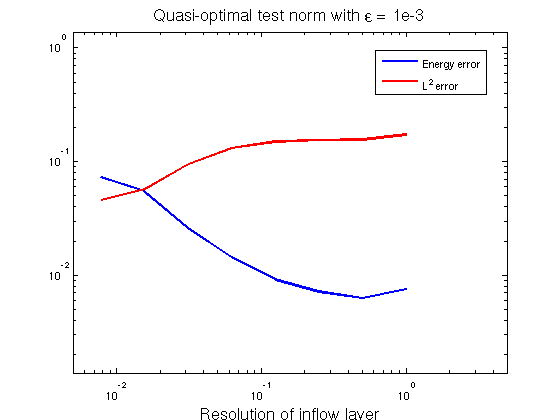
\includegraphics[scale = .35]{figs/qoptInflowDirichlet.png}}
\subfigure{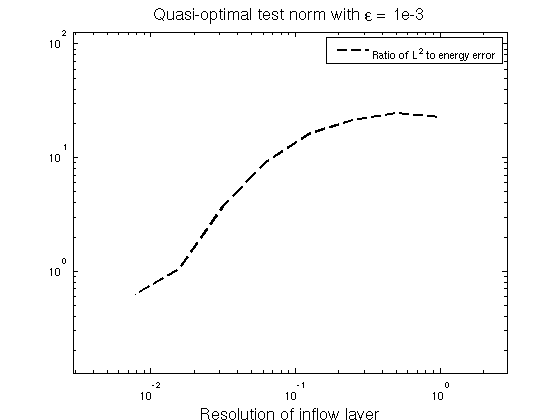
\includegraphics[scale=.35]{figs/qoptInflowDirichletRatio.png}}
%\caption{Energy error and total $L^2$ error and their ratios for different levels of resolution of the inflow layer.}
\end{figure}
}

\frame{
\frametitle{Distribution of error}
We expect that the term $\nor{\div \tau - \beta \cdot \grad v}_{L^2}$ is bounded uniformly in $\epsilon$. However, the term $\nor{\frac{1}{\epsilon}\tau - \grad v}_{L^2}$ is not.\footnote{Analytical calculations in 1D show that this term grows with the Peclet number in the element at the inflow, where the adjoint solution develops a boundary layer.}  

As the boundedness of this term determines the robustness of $\sigma$, our energy norm is
\begin{align*}
\nor{\boldsymbol U}_E &\simeq \sup_{\LRp{v,\tau}}\LRp{\frac{\LRp{u,\Grad_h \cdot \tau - \beta \cdot \Grad_h v}_{\Omega}}{\nor{\LRp{v,\tau}}_V} + \frac{\LRp{\sigma, \frac{1}{\epsilon}\tau + \Grad_h v}_{\Omega}}{\nor{\LRp{v,\tau}}_V}} + \text{etc} \\
&\approx \nor{u}_{L^2} + C_{\text{Pe}}\nor{\sigma}_{L^2} + \nor{\LRp{\uh,\fnh}}
\end{align*}
where $\text{Pe}$ is the element Peclet number near the inflow, and $C_{\text{Pe}}$ accounts for the underresolution of the inflow layer.
%For the quasi-optimal test norm, underresolution of the inflow boundary layer negatively affects only the robustness of $u$. 
}

\frame{
\frametitle{Three levels of test functions}
\begin{itemize}
\item $L^2$ optimal test functions resulting from a global adjoint problem,
\item Global test functions resulting from a global Riesz inversion,
\item Local test functions resulting from local Riesz inversions.
\end{itemize}

Thoughts:
\begin{itemize}
\item The complete local resolution of test functions may not be necessary
\item You can have optimal test functions with boundary layers even when there are none in the global adjoint: resolution of these on a global level may still be necessary to maintain robustness.
\end{itemize}

}


\end{document}
